\section{ParSplice Background}
\label{sec:parsplice}

ParSplice~\cite{perez:jctc20150parsplice} is an accelerated molecular dynamics
(MD) simulation tool developed at LANL. Its phases are depicted in
Figure~\ref{fig:arch-parsplice}:

\begin{enumerate}

  \item splicer tells producers to generate segments (short MD trajectory) in
  states

  \item producers read initial coordinates \{\(x_i,y_i\)\} from database 

  \item producer insert final coordinates for each segment \(s_i\) into database 

  \item repeat
\end{enumerate}

The computation can be parallelized by adding more producers or by adding
workers to parallelize individual producers.  The producers are stateless and
read initial coordinates from the database every time they start
generating segments. Since workers do not maintain their own history, they can
end up reading the same coordinates repeatedly. To mitigate the consequences of such
repeated reads, ParSplice provisions a hierarchy of nodes to act as caches that
sit in front of the persistent database. Producers contact this hierarchy of
caches for their segment coordinates. Writes are stored on each tier and reads
traverse up the hierarchy until they find their data. 

\subsection*{Input Deck}

We use ParSplice to simulate the evolution of metallic nanoparticles that grow
from the vapor phase. As the run progresses, the energy landscape of the system
becomes more complex. Two factors control the number of entries in the
database: the growth rate and the temperature. The growth rate controls how
quickly new atoms are added to the nanoparticle: fast rates lead to
non-equilibrium conditions, and hence increase the number of states that can be
visited. However, as the particle grows, the simulation slows down because the
calculations become more expensive, limiting the rate at which new states are
visited. On the other hand, the temperature controls how easily a trajectory
can jump from state to state; higher temperatures lead to more frequent
transitions.

The nanoparticle simulation stresses the database architecture of ParSplice. It
visits more states than other input decks because the system uses a cheap
potential, has a small number of atoms, and a complex energy landscape with
many accessible states. Changing the growth rate and temperature changes the
size, shape, and locality of the database keyspace. Lower temperatures and
smaller growth rates create hotter keys with smaller keyspaces as many segments
are generated in the same set of states, before the trajectory can escape to a
new region of state space.

Our evaluation uses the total ``trajectory length" as the goodness metric. This
value is the duration of the overall trajectory produced by the system. At
ideal efficiency, the trajectory length should increase with the square root of
the wall-clock time, since the wall-clock cost of timestepping the system by
one simulation time unit increases in proportion of the total number of atoms,
and hence of the total simulation time thus far. 


\begin{figure}[t]
  \noindent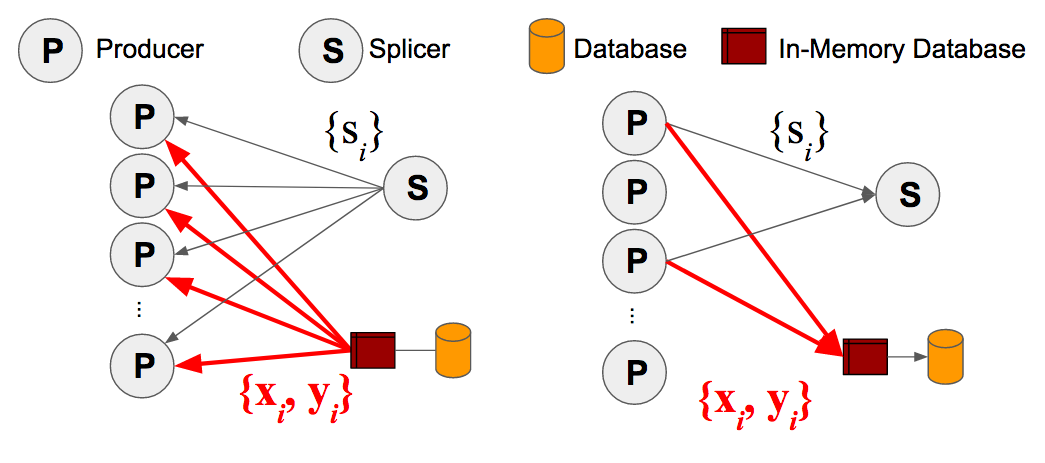
\includegraphics[width=19pc,angle=0]{figures/arch-parsplice.png}\\
  \caption{ParSplice is a read-heavy HPC application where producers use a
  database for consistency. \label{fig:arch-parsplice}}
\end{figure}

